\documentclass[12pt, dutch, a4paper]{article}

\usepackage[hidelinks]{hyperref}
\usepackage[tmargin=0.8in, bmargin=1in]{geometry}
\usepackage{parskip}
\usepackage{amssymb}
\usepackage{amsmath}
\usepackage[shortlabels]{enumitem}
\usepackage[dutch]{babel}
\selectlanguage{dutch}
\usepackage{amsthm}
\usepackage{cleveref}
\usepackage{graphicx}
\usepackage{siunitx}

\theoremstyle{definition}

\newtheorem{theorem}{Stelling}
\newtheorem{lemma}{Lemma}[theorem]
\newtheorem{lemmalos}{Lemma}
\newtheorem{sublemma}{Lemma}[lemma]
\newtheorem{case}{Geval}
\newtheorem{claim}{Claim}

\newenvironment{shortclaim}
  {\refstepcounter{claim}\textbf{Claim~\theclaim.}}% \begin{shortthm}
{\enskip}
\newenvironment{shortthm}
  {\refstepcounter{theorem}\textbf{Stelling~\thetheorem.}}% \begin{shortthm}
{\enskip}

\usepackage[newfloat]{minted}
\usepackage{caption}

\newenvironment{code}{\captionsetup{type=listing}}{}
\SetupFloatingEnvironment{listing}{placement=htp}
\SetupFloatingEnvironment{listing}{name=Code blok}

\title{Data Py - inleveropdracht 1}
\author{Boris van Boxtel, Brechtje Poppen, \\  Floris Oostenbrug, Lotte Gritter}
\date{23 December 2022 - Week 51} 

\begin{document}

\maketitle  
\pagenumbering{arabic} 

\subsection*{Fourierreeksen}



\subsection*{Testfuncties}
\subsection*{Convergentie}
\begin{enumerate}[(a)., wide]
  \item
  Vanaf nu is de variabelen $f_0$ gelijk aan 1. Gegeven is dat de coëfficiënten van de Fourierreeks van de driehoeksgolf gegeven worden door:
  \begin{equation} \label{trianglewave}
    A_n = \frac{8}{\pi^2} 
    \begin{cases}
      0 & n \text{ even} \\
      \frac{(-1)^{ (n-1)/2 }}{n^2} & n \text{ oneven}
    \end{cases}.
  \end{equation}
  We berekenen de eerste $n$ van deze coëfficiënten van de driehoeksgolf met de volgende python code:
  % \begin{code}
  %   \inputminted[
  %     firstline=43,
  %     lastline=50,
  %     frame=lines, 
  %     breaklines,
  %     linenos,
  %     ]{python}{code/Data_py_week_5.py}
  %   \caption{Code voor het genereren van de coëfficiënten bij \cref{trianglewave}}
  % \end{code}

  Ook is gegeven dat de coëfficiënten van de Fourierreeks van de zaagtandgolf gegeven worden door:
  \begin{equation} \label{sawtooth}
    A_0 = 0 \quad A_{n > 0} = -\frac{1}{\pi n}.
  \end{equation}
  We berekenen de eerste $n$ van de coëfficiënten van de zaagtandgolf met de volgende python code:

  \newpage
  % \begin{code}
  %   \inputminted[
  %     firstline=53,
  %     lastline=58,
  %     frame=lines, 
  %     breaklines,
  %     linenos,
  %     ]{python}{code/Data_py_week_5.py}
  %   \caption{Code voor het genereren van de coëfficiënten bij \cref{sawtooth}}
  % \end{code}

  We kunnen met deze functies en de volgende code een illustratie maken van de Fourier transform van de driehoeksgolf:
  % \begin{code}
  %   \inputminted[
  %     firstline=69,
  %     lastline=95,
  %     frame=lines, 
  %     breaklines,
  %     linenos,
  %     ]{python}{code/Data_py_week_5.py}
  %   \caption{Code voor het genereren van Figuur 1}
  % \end{code}

  Het plaatje dat hiermee wordt gegenereerd is het volgende:
  \begin{figure}[h] \label{driehoekfiguur}
    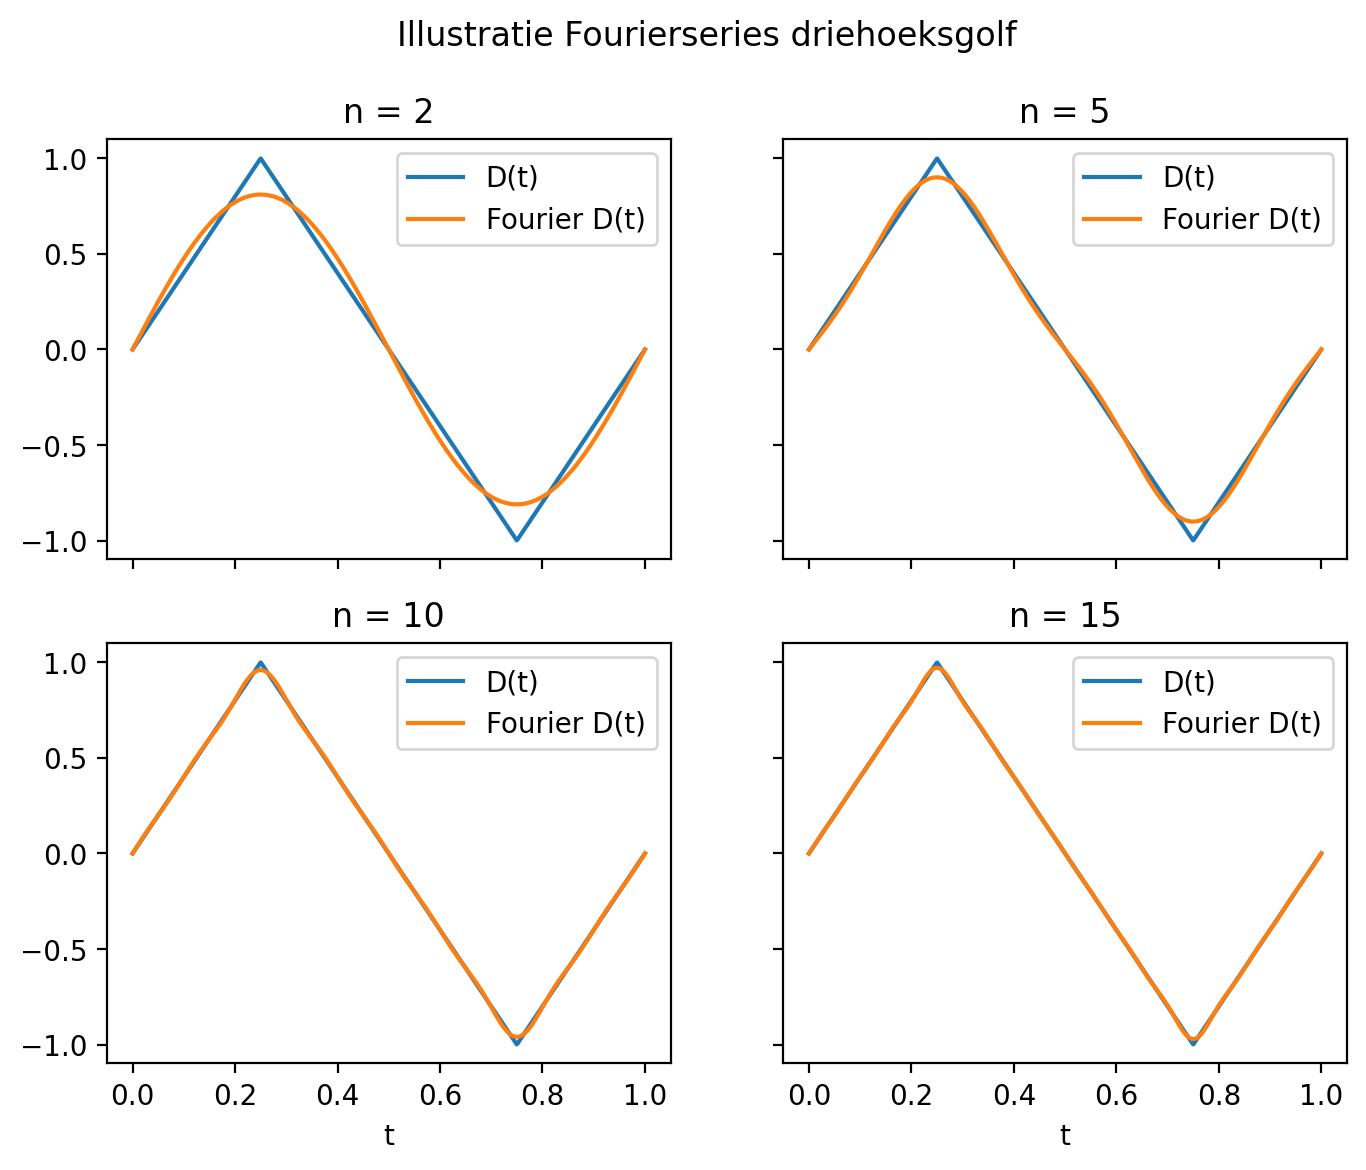
\includegraphics[width=\textwidth]{images/Fourier_driehoekgolf.png}
    \caption{Illustratie van Fouriertransformatie driehoeksgolf}  
  \end{figure}

  \newpage
  We kunnen met vergelijkbare code een plaatje maken voor de zaagtandgolf:
  \begin{figure}[h] \label{zaagtandfiguur}
    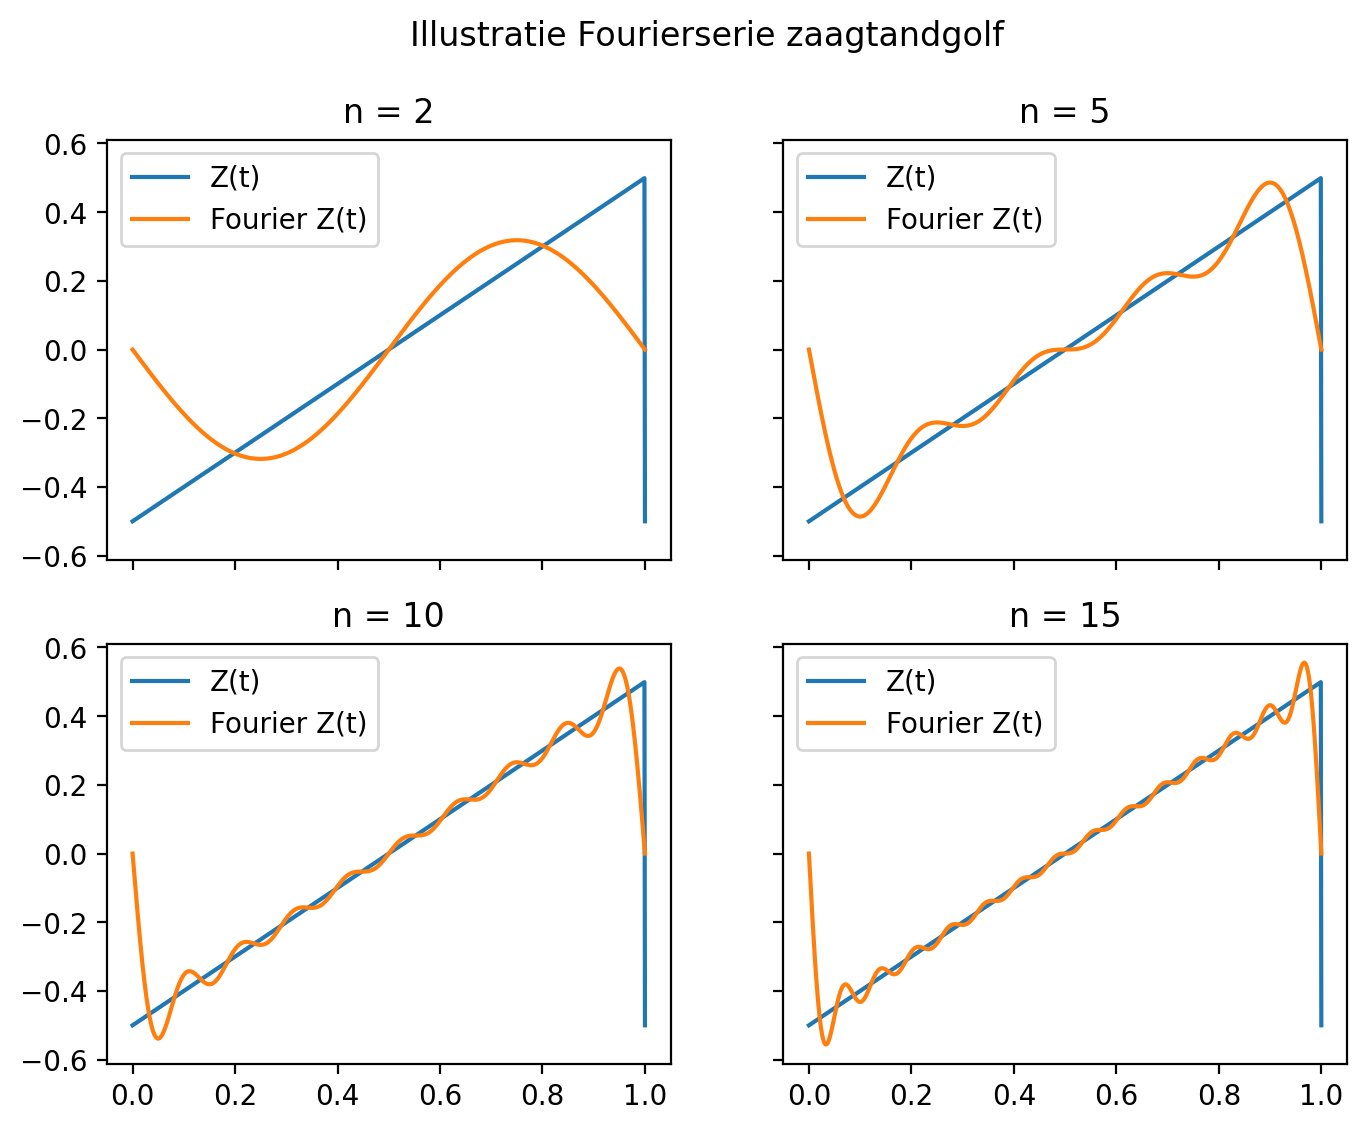
\includegraphics[width=\textwidth]{images/Fourier_zaagtandgolf.png}
    \caption{Illustratie van Fouriertransformatie zaagtandgolf}  
  \end{figure}
  \item
  We gebruiken de volgende functie om het totale kwadratische verschil van twee array's te berekenen:
  % \begin{code}
  %   \inputminted[
  %     firstline=59,
  %     lastline=65,
  %     frame=lines, 
  %     breaklines,
  %     linenos,
  %     ]{python}{code/Data_py_week_5.py}
  %   \caption{Code voor het berekenen van het totale kwadratische verschil}
  % \end{code}
  We vinden het totale kwadratische verschil van bijvoorbeeld de driehoeksgolf met zijn Fourier transform met 2 coëfficiënten als volgt:
  % \begin{code}
  %   \inputminted[
  %     firstline=130,
  %     lastline=130,
  %     frame=lines, 
  %     breaklines,
  %     linenos,
  %     ]{python}{code/Data_py_week_5.py}
  % \end{code}

  Deze code geeft de volgende waarden voor de totale kwadratische verschillen voor een verschillend aantal Fourier coëfficiënten $n$:

  \begin{figure}[h]
    \begin{minipage}[c]{0.49\linewidth}
      \centering
      \caption*{Driehoeksgolf}
      \begin{tabular}{c | c}
        $n$ & totaal kwadratisch verschil \\
        \hline
        2   & 4.817 \\
        5   & 0.765 \\
        10  & 0.054 \\
        15  & 0.020 \\
      \end{tabular}
    \end{minipage} 
    \hfill
    \begin{minipage}[c]{0.49\linewidth}
      \centering
      \caption*{Zaagtandgolf}
      \begin{tabular}{c | c}
        $n$ & totaal kwadratisch verschil \\
        \hline
        2   & 32.89 \\
        5   & 11.45 \\
        10  & 5.576 \\
        15  & 3.744 \\
      \end{tabular}
    \end{minipage}
  \end{figure}

  We zien in de plots bij de driehoeksgolf dat deze bij hetzelfde aantal Fourier coëfficiënten "dichter" bij de echte functie is dan de zaagtandgolf. Dit zien we vervolgens direct ook terug in de zojuist berekende kwadratische verschillen; deze zijn namelijk bij de zaagtandgolf een stuk groter.

  \item
  Tot slot kunnen we met de volgende code de totale kwadratische verschillen van zowel de driehoeksgolf als de zaagtandgolf weergeven. We kunnen hier helaas geen gebruik maken van numpy's vermogen om met array's te rekenen, dus we maken gebruik van een for loop.
  % \begin{code}
  %   \inputminted[
  %     firstline=141,
  %     lastline=157,
  %     frame=lines, 
  %     breaklines,
  %     linenos,
  %     ]{python}{code/Data_py_week_5.py}
  % \end{code}

  De figuur is het volgende:
  \begin{figure}[h]
    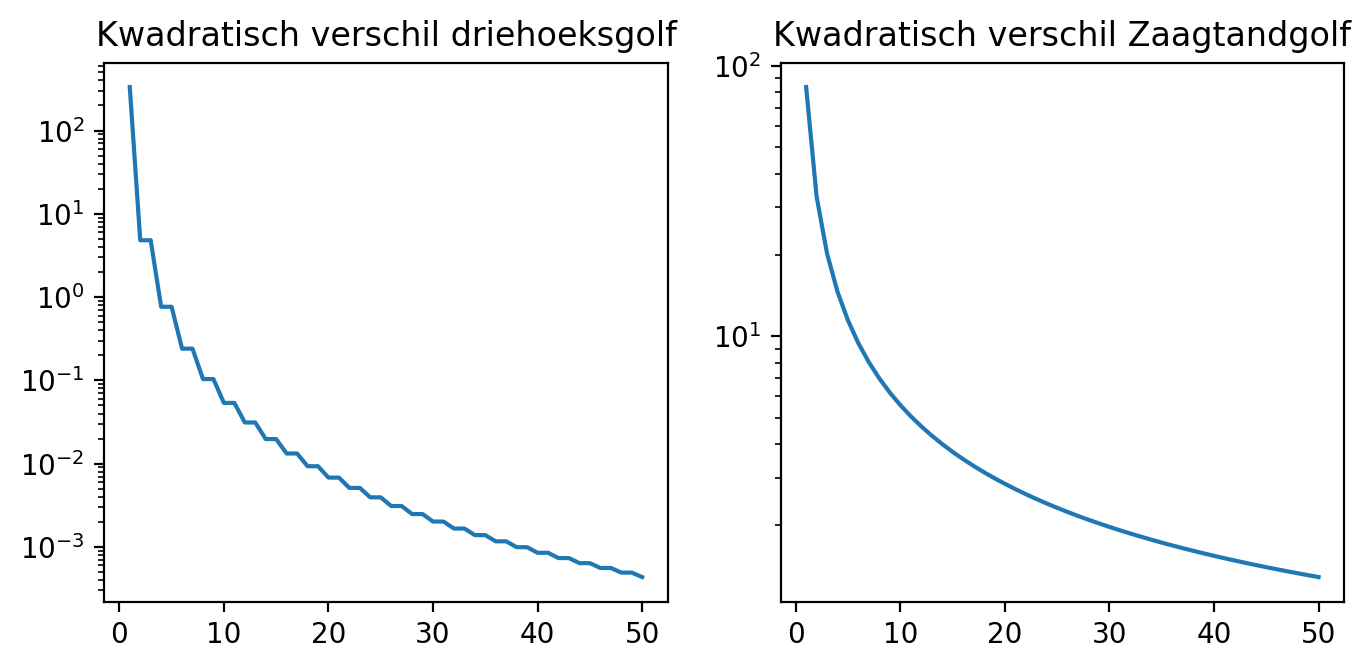
\includegraphics[width=\textwidth]{images/tot_kwadratisch_verschil.png}
    \caption{Kwadratisch verschil op de y-as tegen het aantal coëfficiënten op de x-as}
  \end{figure}
\end{enumerate}
\subsection*{Conclusies}



\end{document}